\documentclass{rapport}
\usepackage{lipsum}
\usepackage{gensymb}
\usepackage{float}
\usepackage{graphicx} % Required for inserting images
\usepackage{amsmath}
\usepackage{amsfonts}
\usepackage{wrapfig}
\usepackage{afterpage}




\usepackage{listings}
\lstset{
    basicstyle=\ttfamily\small,
    keywordstyle=\color{blue},
    commentstyle=\color{gray},
    stringstyle=\color{red},
    showstringspaces=false,
    breaklines=true
}

\usepackage{pgfplots}
\pgfplotsset{compat=1.18}

\title{Crittografia} %title of the file

\begin{document}

%----------- Report information ---------

\logo{logos/logo.jpg}
\uni{\textbf{Newton-Pertini di Camposampiero}}
\ttitle{Crittografia} %title of the file
\subject{Sistemi e Reti} % Subject name
\topic{Crittografia} % Topic name

\professor{Gianfranco \textsc{Lamon}} % information related to the professor

\students{Alex Gasparini} % information related to the students

%----------- Init -------------------
        
\buildmargins % display margins
\buildcover % create the front cover of the document
\toc % creates the table of contents

%------------ Report body ----------------


\paragraph{Introduzione}
In questo corso vedremo le basi della \textbf{crittografia}, analizzando anche minuziosamente alcuni aspetti. La crittografia è quella branca della matematica e dell'informatica che studia come inviare messaggi e informazioni in modo che non siano comprensibili o leggibili da chi non è il mittente o il destinatario del messaggio. Inizieremo da una crittografia "semplice": \textbf{One Time Pad} (spesso abbreviato in \textbf{OTP}), con "semplice" intendo dire che per comprenderlo non sono necessarie conoscenze preliminari. D'altro canto, le altre tecniche che vedremo si basano su una solida base matematica, molto complessa, ma riprenderemo anche queste nozioni matematiche. In particolare, esamineremo nel dettaglio gli algoritmi \textbf{RSA} e \textbf{Diffie-Hellman}, che hanno due funzionalità ben distinte ma sono comunque pietre miliari della crittografia moderna. In entrambe le tecniche analizzeremo anche le dimostrazioni e forniremo esempi pratici per comprendere a fondo questo argomento, che, pur essendo apparentemente difficile, affascina per le sue applicazioni nella vita reale.

\section{Crittografia: introduzione e prime definizioni}


\section{Cifrati Antichi - Cifrario di Cesare}



\newpage

\section{Cifrati Antichi - Enigma}

\begin{wrapfigure}{r}{0.35\textwidth}
    \centering
    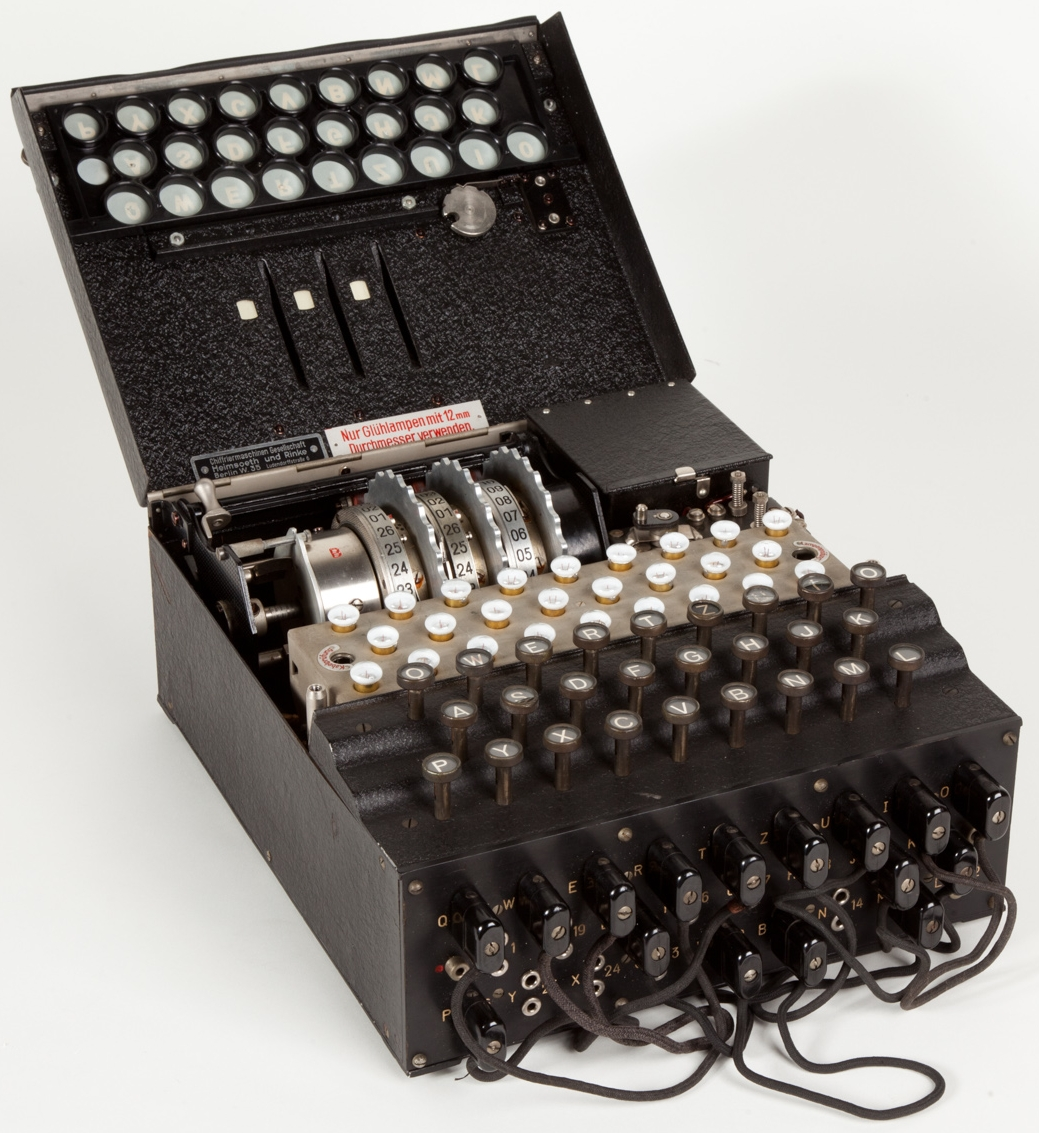
\includegraphics[width=0.30\textwidth]{logos/enigma.jpg}
    \caption*{Foto della macchina Enigma}
\end{wrapfigure}

La tecnica \textbf{OTP}, per come l'abbiamo studiata fino ad ora, è utilizzabile solo tramite i computer, ma in realtà è molto più antica e, durante la \textbf{Seconda Guerra Mondiale}, ha giocato un ruolo fondamentale. Infatti, i tedeschi hanno utilizzato la \textbf{Macchina Enigma}, che permetteva loro di comunicare inviando messaggi cifrati. La macchina Enigma, per l'appunto, usa una tecnica di crittografia molto simile, se non uguale, all'\textbf{OTP}.


\subsection{Preambolo Storico}

La macchina Enigma è stata brevettata da \textbf{Arthur Scherbius}, un ingegnere tedesco, nel \textbf{1918}. Al contrario di quanto si pensa, Enigma veniva utilizzata anche prima della Seconda Guerra Mondiale, soprattutto dalla \textbf{marina militare tedesca}. Tuttavia, Enigma ha avuto un ruolo importantissimo durante la Seconda Guerra Mondiale, perché ha permesso ai tedeschi di inviare messaggi sicuri, impedendo agli Alleati di comprendere le decisioni militari tedesche. 

La macchina Enigma aveva una \textbf{chiave privata} (che vedremo in dettaglio più avanti) che veniva cambiata \textbf{ogni giorno a mezzanotte}. La chiave veniva inviata soltanto agli ufficiali tedeschi di grado più alto per evitare fughe di informazioni riservate. Infatti, verso mezzanotte, ai generali tedeschi arrivava un messaggio chiamato \textbf{Schlüsselheft}, che conteneva la chiave del giorno. In realtà, alcuni reparti tedeschi, come la marina militare, che richiedevano maggiore sicurezza, cambiavano chiave ogni \textbf{8 ore}. Inoltre, erano previsti protocolli di sicurezza, come il fatto che il \textbf{Schlüsselheft} dovesse essere conservato in un luogo sicuro sotto chiave, con accesso riservato solo a poche persone autorizzate. Se vi era il rischio che gli Alleati potessero entrarne in possesso, il \textbf{Schlüsselheft} doveva essere immediatamente distrutto tramite il fuoco.

\subsection{Funzionamento}

La macchina Enigma serviva per crittografare e decrittografare i messaggi. Era dotata di una tastiera e, alla pressione di un tasto (dove ogni tasto rappresentava una lettera dell'alfabeto tedesco), si accendeva un led che indicava un'altra lettera dell'alfabeto. Per utilizzare una macchina Enigma, di solito erano necessarie due persone: una che scriveva il messaggio da cifrare o decifrare e un'altra che annotava le lettere che si illuminavano.

\begin{wrapfigure}{l}{0.35\textwidth}
    \centering
    \vspace{-1.5cm}
    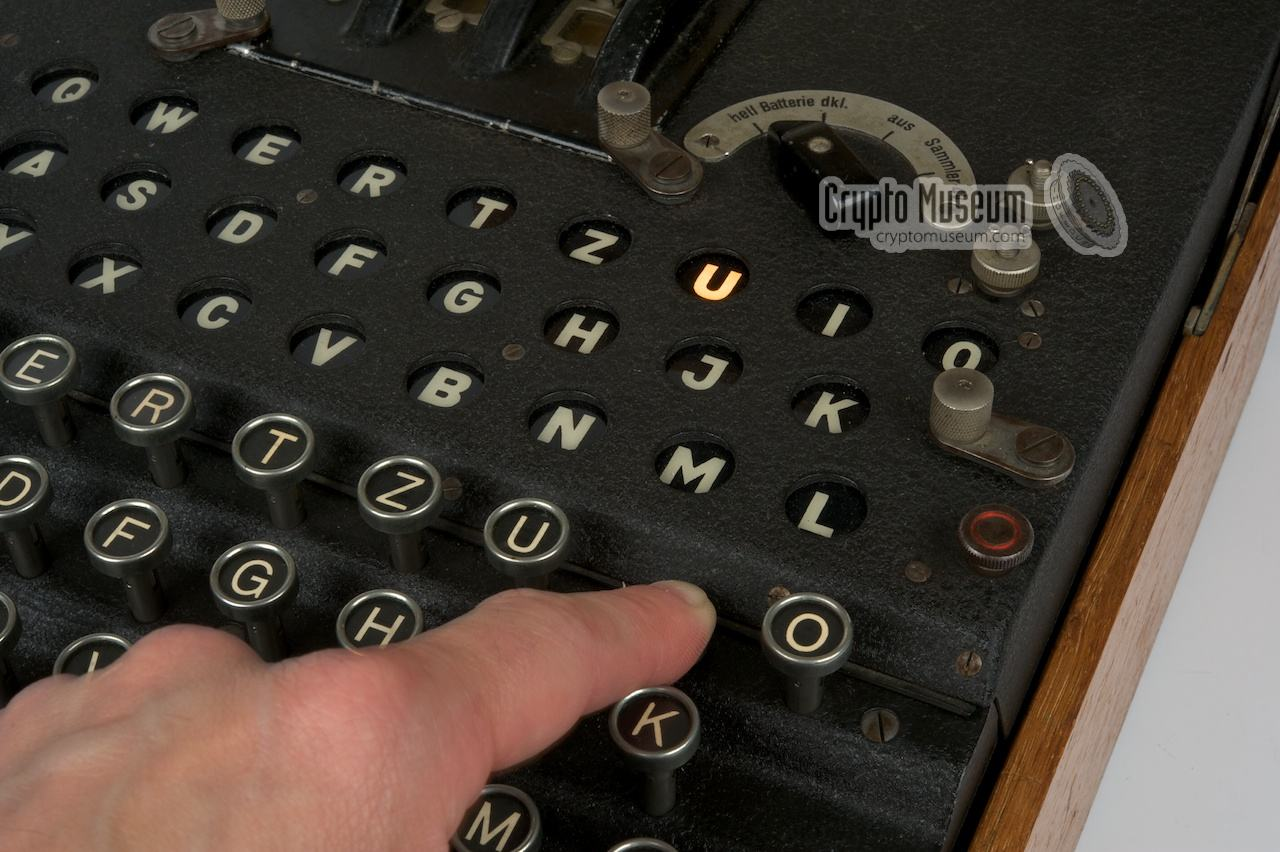
\includegraphics[width=0.35\textwidth]{logos/enigma2.jpg}
\end{wrapfigure}

\vspace{+1.5cm}

Nell'immagine possiamo notare che, alla pressione del tasto \textbf{I} sulla tastiera, si illumina la lettera \textbf{U} nella parte superiore.

\afterpage{\clearpage}



\newpage
\subsection{Struttura}

Ogni macchina Enigma era composta da sei parti principali: \textbf{Tastiera}, \textbf{Rotori}, \textbf{Riflettore}, \textbf{Lampboard}, \textbf{Plugboard} e la \textbf{Batteria}.  

Partiamo dagli elementi più semplici: la batteria serviva ad alimentare la parte elettrica della macchina, mentre la tastiera conteneva le 26 lettere dell'alfabeto sotto forma di pulsanti. La tastiera funzionava in modo simile a quelle odierne, nel senso che, alla pressione di un tasto, si chiudeva il circuito elettrico.  

La \textbf{Lampboard} (detta \textbf{Lampenbrett} in tedesco) era la parte in cui si trovavano le lettere che si illuminavano alla pressione dei tasti sulla tastiera.  

\subsubsection{Plugboard}

La \textbf{Plugboard} (detta anche \textbf{Steckerbrett}) serviva per invertire una coppia di lettere. Questa inversione avveniva sia in input (quindi prima di eseguire l'algoritmo di cifratura) sia in output (dopo aver cifrato il messaggio). Questa caratteristica serviva esclusivamente ad aggiungere un ulteriore livello di sicurezza, ma non era il punto focale della macchina.

\begin{figure}[h]
    \centering
    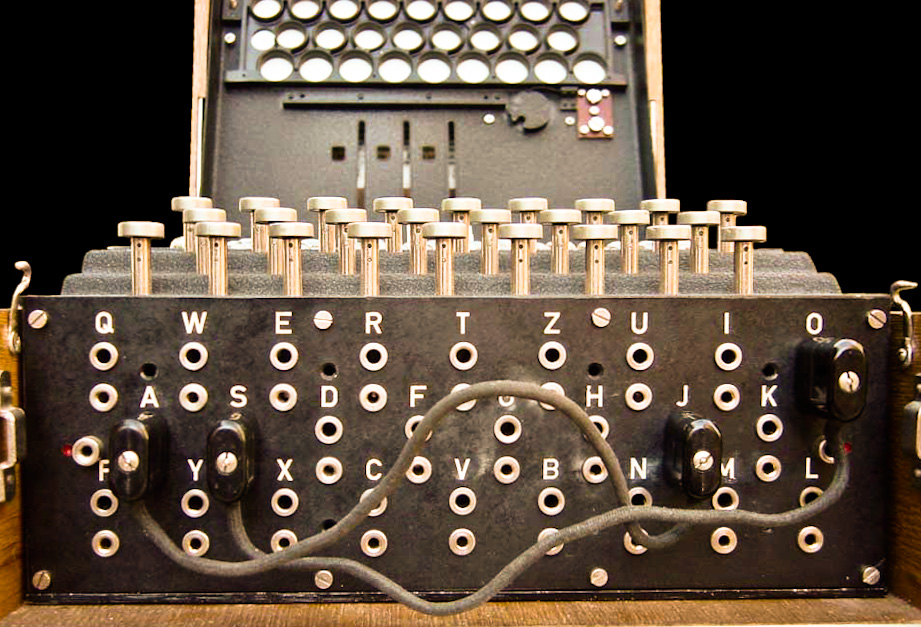
\includegraphics[width=0.6\linewidth]{logos/enigma3.jpg}
\end{figure}

Nell'immagine possiamo notare come siano collegate le coppie (\textbf{A}, \textbf{J}) e (\textbf{S}, \textbf{O}).  
Quindi, se veniva premuto il tasto \textbf{A} sulla tastiera, esso veniva prima trasformato in \textbf{J}, che poi seguiva il resto dell'algoritmo.  
Allo stesso modo, se la lettera crittata era \textbf{S}, questa veniva cambiata in \textbf{O}, e quindi si illuminava la lettera \textbf{O} sulla lampboard.

\subsubsection{Rotori}

\begin{wrapfigure}{r}{0.35\textwidth}
    \vspace{-1cm}
    \centering
    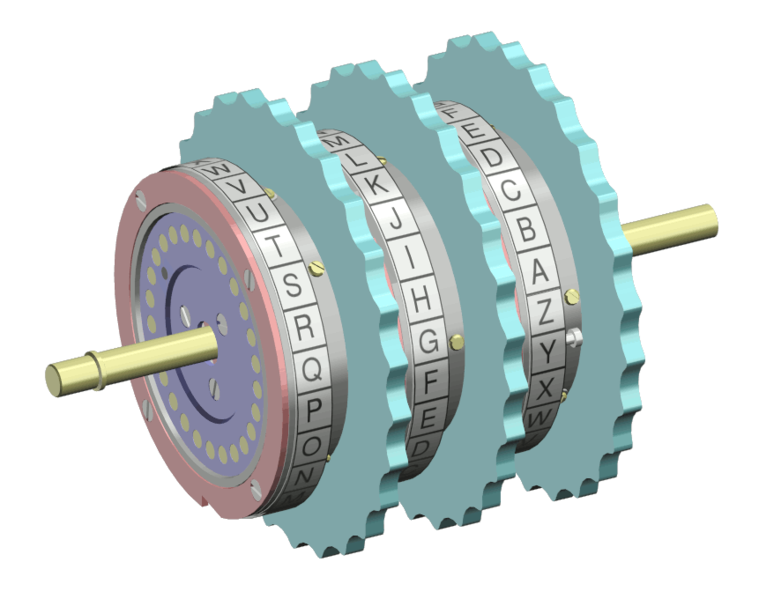
\includegraphics[width=0.35\textwidth]{logos/enigma5.png}
    \caption*{Render 3D di tre rotori collegati}
\end{wrapfigure}

La parte principale dell'algoritmo di cifratura sono \textbf{i rotori}, che permettono di trasformare le lettere per crittarle.  
Un rotore è un componente metallico circolare collegato a un ingranaggio che gli permette di ruotare e cambiare lettera, come vedremo in seguito.  
Inoltre, è montato su un asse che ne consente la rotazione e, su entrambi i lati, presenta 26 punti di contatto metallici che permettono di trasmettere la corrente tra un rotore e l'altro.

\afterpage{\clearpage}   


\newpage
Per comprendere meglio il funzionamento di un rotore, è utile analizzarne la struttura interna:

\begin{figure}[h]
    \centering
    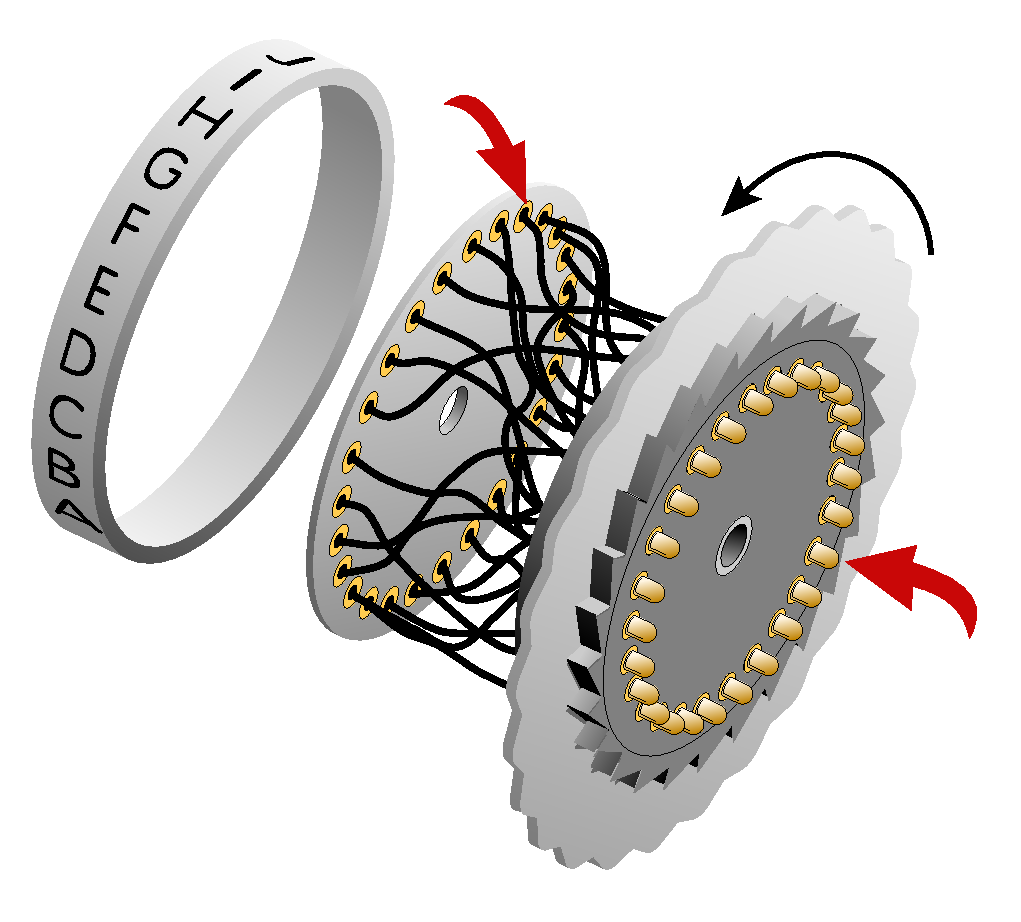
\includegraphics[width=0.6\linewidth]{logos/Mediamodifier-Design-ritagliato.pdf}
\end{figure}

Come accennato in precedenza, entrambi i lati del rotore presentano piastre metalliche per la conduzione della corrente (indicate dalla freccia rossa nell'immagine). Inoltre, ogni punto di contatto su un lato è collegato a un punto sull'altro lato, ma in modo disordinato. Questo collegamento permette di mescolare le lettere: una lettera che "entra" nel rotore ne "uscirà" come un'altra, a causa di questo rimescolamento.  

Di norma, una macchina Enigma contiene tre rotori collegati in serie per aumentare la complessità della cifratura. Tuttavia, alcune versioni della macchina Enigma utilizzano quattro o più rotori, semplicemente per incrementare la sicurezza e rendere ancora più difficile la decrittazione.





\subsubsection{Riflettore}
\begin{wrapfigure}{r}{0.35\textwidth}
    \vspace{-1cm}
    \centering
    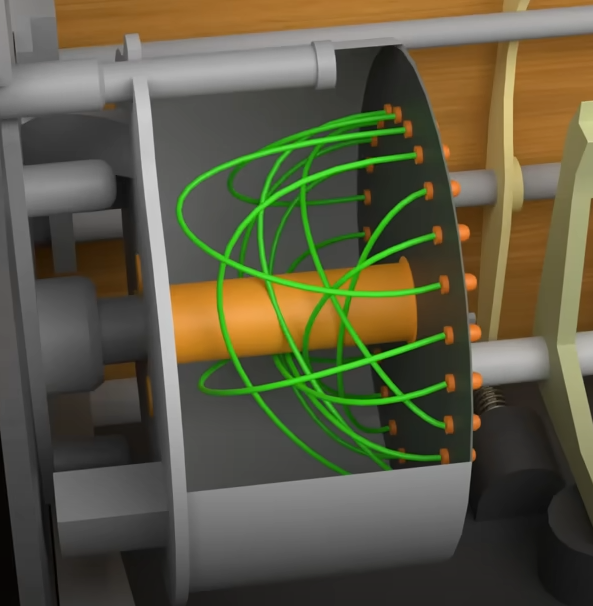
\includegraphics[width=0.35\textwidth]{logos/Screenshot from 2025-02-10 17-26-46.png}
    \caption*{Render 3D di un Riflettore}
\end{wrapfigure}

Per aumentare ulteriormente la sicurezza, i tre rotori sono collegati a un \textbf{Riflettore}, il quale fa "rientrare" il segnale nei rotori, permettendo un'ulteriore trasformazione delle lettere. Questo avviene perché la corrente attraversa nuovamente tutti e tre i rotori in senso inverso.

In questo modo, una lettera viene cifrata \textbf{sei volte} prima di essere visualizzata sulla lampboard.

\afterpage{\clearpage}  


\newpage
\subsection{Funzionamento}
Ripercorriamo il funzionamento della macchina Enigma. 

\begin{figure}[h]
    \centering
    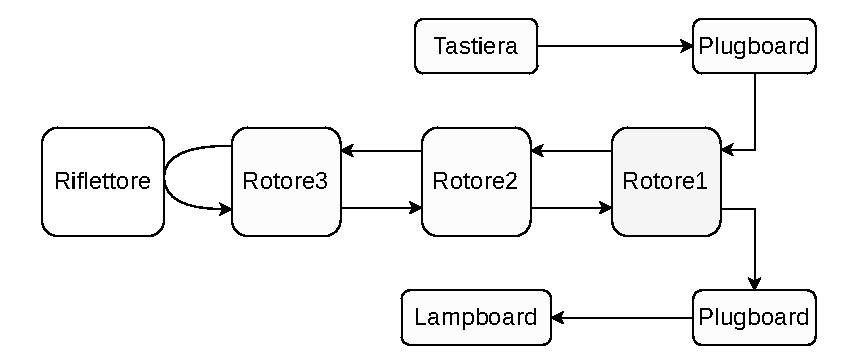
\includegraphics[width=0.9\linewidth]{logos/enigma7.pdf}
\end{figure}

Quando viene premuto un tasto sulla \textbf{Tastiera}, il segnale passa attraverso la \textbf{Plugboard}, che sostituisce la lettera con quella associata se un cavo è collegato; altrimenti, il segnale prosegue direttamente verso i \textbf{Rotori}. Successivamente, attraversa i tre rotori, modificando la lettera tre volte. Grazie al \textbf{Riflettore}, il segnale viene reinviato attraverso i rotori, che trasformano nuovamente la lettera per altre tre volte. Infine, il segnale passa nuovamente per la \textbf{Plugboard}, che può applicare un'ulteriore sostituzione se la lettera è collegata a un'altra. Dopo tutte queste trasformazioni, la lettera finale viene visualizzata sulla \textbf{Lampboard}. 

Durante questo processo, la lettera viene trasformata un minimo di \textbf{6 volte} e fino a un massimo di \textbf{8 volte} se la \textbf{Plugboard} modifica sia l'input che l'output.

Non appena il tasto premuto viene rilasciato, il primo rotore ruota di una posizione grazie a un ingranaggio, modificando così la configurazione delle lettere. Questo meccanismo assicura che, anche premendo due volte di seguito la stessa lettera, vengano visualizzate lettere completamente diverse, poiché la rotazione del rotore cambia continuamente le combinazioni possibili. 

\begin{figure}[h]
    \centering
    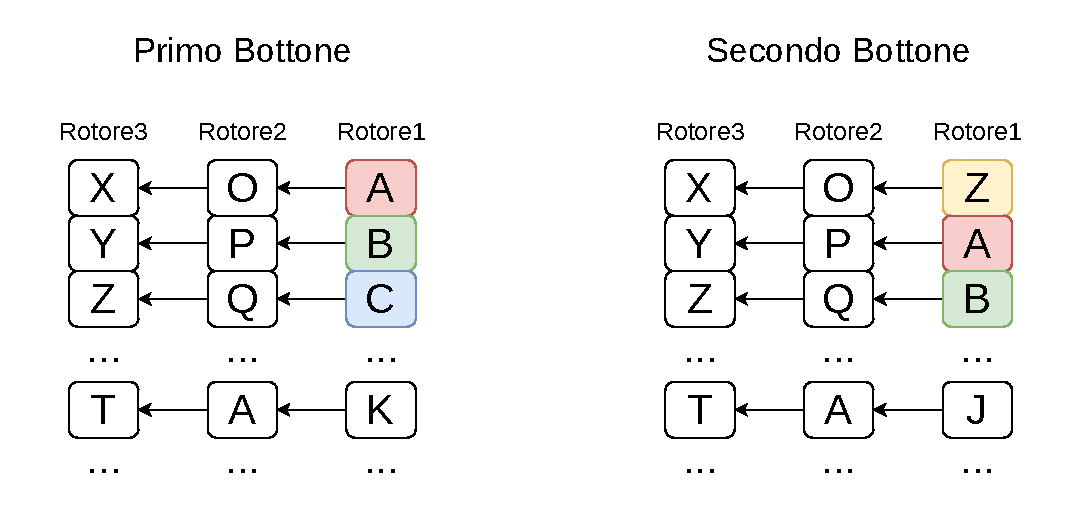
\includegraphics[width=\linewidth]{logos/enigma8.pdf}
\end{figure}


\section{One Time Pad}
La prima forma di crittografia che vediamo è \textbf{One Time Pad}, che è una crittografia \textbf{Simmetrica}. Con il termine crittografia simmetrica si intendono tutte le tecnite crittografiche che usano una sola chiave per criptare e decriptare, al contrario della crittografia asimmetrica che ne usa due, ma questo lo vedremo bene più avanti. Prima di capire bene il funzionamento di questa tecnica è meglio rivedere cos'è lo \textbf{XOR} e come funziona.


\subsection{XOR}
Lo \textbf{XOR} (\textit{eXclusive OR}) è un operatore booleano binario la cui tabella di verità è la seguente:

\begin{center}
\begin{table}[h]
\centering
\begin{tabular}{c|c|c}
A & B & XOR(A, B) \\
\hline
0 & 0 & 0         \\
0 & 1 & 1         \\
1 & 0 & 1         \\
1 & 1 & 0         \\
\end{tabular}
\end{table}
\end{center}

Per ricordarla a memoria, basta sapere che, se A e B sono diversi, lo XOR restituisce 1; altrimenti, se sono uguali, restituisce 0.

Ci interessano in particolare le seguenti proprietà dello XOR:

\begin{equation*} (A \oplus B) \oplus B = A \end{equation*}

\begin{equation*} A \oplus 0 = A \end{equation*}

dove $\oplus$ è il simbolo dello XOR. In realtà, queste proprietà sono tutto ciò che ci serve per comprendere il nostro algoritmo crittografico, quindi passiamo ad analizzarne il funzionamento.















\newpage
\subsection{Funzionamento}
L'algoritmo \textbf{OTP} inizia generando una chiave lunga almeno quanto il messaggio da cifrare. La chiave può assumere qualsiasi forma, purché sia privata e nessuno la conosca. Dopo la generazione della chiave, è sufficiente XORarla con il messaggio che vogliamo inviare:  

\begin{equation*}
    C = M \oplus K 
\end{equation*}

dove \(C\) è il messaggio cifrato (\textit{Crypted message}), \(M\) è il messaggio originale (\textit{Message}) e \(K\) è la chiave (\textit{Key}).  

Una volta inviato il messaggio, il destinatario può semplicemente applicare l'operazione XOR tra il messaggio ricevuto e la chiave per recuperare il messaggio originale:  

\begin{equation*}
   C \oplus K
\end{equation*}

Per capire perché il metodo funziona, sostituiamo l'equazione precedente (\(C = M \oplus K\)):  

\begin{equation*}
    (M \oplus K) \oplus K
\end{equation*}

Utilizzando la proprietà dello XOR, otteniamo:  

\begin{equation*}
    M = (M \oplus K) \oplus K 
\end{equation*}

In questo modo, applicando l'operazione XOR, recuperiamo esattamente il messaggio originale.  














\begin{figure}[h]
    \centering
    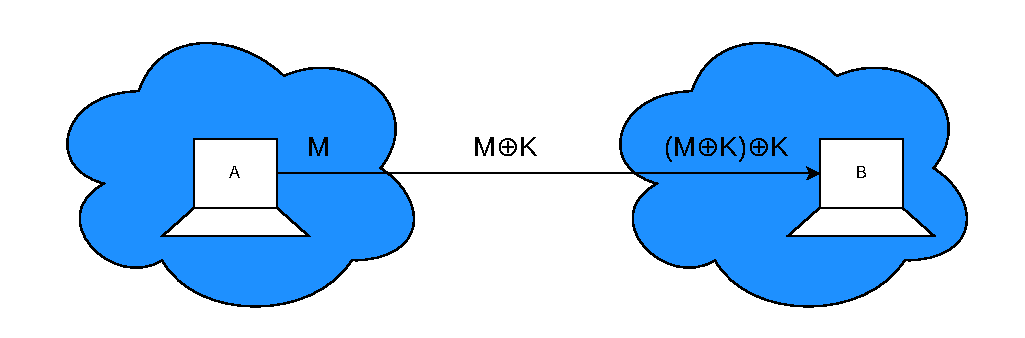
\includegraphics[width=0.9\linewidth]{logos/crit5.pdf}
\end{figure}


\subsubsection{Considerazioni}

Questo algoritmo, però, non si occupa della condivisione sicura della chiave. Per questo scopo si può utilizzare l'algoritmo \textbf{Diffie-Hellman}, che è progettato proprio per condividere chiavi private in modo sicuro.  

La forza e la bellezza di questo algoritmo risiedono nel fatto che è \textbf{completamente sicuro}: è stato infatti dimostrato matematicamente che è impossibile decifrare il messaggio cifrato (\(M \oplus K\)) senza conoscere la chiave. L'\textbf{OTP} è, infatti, l'unico algoritmo \textbf{impossibile da decifrare} e completamente sicuro che conosciamo al momento. L'unico metodo per indovinare il messaggio è tentare casualmente e sperare in un colpo di fortuna.  

Ovviamente, non è tutto oro ciò che luccica: se fosse davvero perfetto, useremmo solo questa tecnica e saremmo al 100\% sicuri. Tuttavia, come vedremo, questo algoritmo presenta un problema non da poco.  




\subsection{Crackabilità}
Il problema di questa tecnica risiede nel nome: \textbf{ONE TIME Pad}. Ovvero, questa tecnica si può usare \textbf{una sola volta} con la stessa chiave. Questo è un requisito fondamentale, perché qualora una chiave venga usata più di una volta, tramite varie tecniche si può estrapolare la chiave e i messaggi, almeno parzialmente.  

Questo accade perché, dati due messaggi in chiaro (\(\mathbf{M_1}\), \(\mathbf{M_2}\)), una chiave privata (\(\mathbf{K}\)) e le loro combinazioni cifrate (\(\mathbf{C_1}\), \(\mathbf{C_2}\)):  

\begin{equation*}
    C_1 = M_1 \oplus K 
\end{equation*}
\begin{equation*}
    C_2 = M_2 \oplus K    
\end{equation*}

Supponiamo di aver intercettato i messaggi cifrati: possiamo applicare l'operazione XOR tra di loro:  

\begin{equation*}
    C_1 \oplus C_2
\end{equation*}

Riscriviamo l'espressione sostituendo i valori di \(C_1\) e \(C_2\):  

\begin{equation*}
    C_1 \oplus C_2 = (M_1 \oplus K ) \oplus (M_2 \oplus K)
\end{equation*}

Ora, grazie alla proprietà associativa dello XOR, possiamo riorganizzare i termini:  

\begin{equation*}
    C_1 \oplus C_2 = (M_1 \oplus M_2 ) \oplus (K \oplus K)
\end{equation*}

Poiché \(K \oplus K = 0\), otteniamo:  

\begin{equation*}
    C_1 \oplus C_2 = (M_1 \oplus M_2 ) \oplus 0
\end{equation*}

Infine, ricordando che \(X \oplus 0 = X\), il risultato finale è:  

\begin{equation*}
    C_1 \oplus C_2 = M_1 \oplus M_2 
\end{equation*}




Dopo tutti questi passaggi, abbiamo scoperto che la XOR tra i due messaggi cifrati è uguale alla XOR dei due messaggi in chiaro. In questo modo, siamo riusciti a "rimuovere" la chiave. Chiaramente, con la XOR dei messaggi in chiaro, comunque non riusciamo a decriptarli, ma possiamo dedurre alcune parti. Infatti, esistono alcuni algoritmi, come \textbf{crib drag}, che, dati alcuni messaggi cifrati, possono decifrare parti dei messaggi e della chiave. Questi algoritmi sono particolarmente complessi e sfruttano certi pattern nelle frasi (come banalmente gli spazi, oppure gli articoli nelle varie lingue) e anche degli \textbf{attacchi con dizionario} (dictionary attack). Per capirli bene e in maniera pratica, consiglio di scaricare i seguenti script Python: \href{https://github.com/CameronLonsdale/MTP}{\textcolor{blue}{\underline{https://github.com/CameronLonsdale/MTP}}}. Inoltre, per gli amanti del rap, vi lascio un esempio divertente per cercare di capire quale canzone è: \href{https://drive.google.com/file/d/1TlU_iIYm5XfBpwMUKk1Ko-MEZ41LIxuF/view?usp=sharing}{\textcolor{blue}{\underline{Link Drive}}}.



\newpage
\section{Cifrari a Blocchi - DES}


\section{Cifrari a Blocchi - AES}



\newpage
\section{RSA}
Nel 1977 i crittografi \textbf{Ronald Rivest}, \textbf{Adi Shamir} e \textbf{Leonard Adleman} inventarono l'algoritmo \textbf{RSA} (dove RSA è l'acronimo dei cognomi dei 3 crittografi). L'RSA è un algortimo per generare una coppia di chiavi private e pubbliche, quindi per definizione rientra nella crittografia asimmetrica. RSA si occupa solo di generare le chiavi, ma non si occupa di condividere privatamente la chiave privata, per quello vedremo l'algoritmo di \textbf{Diffie-Hellman}.


\subsection{Funzionamento Generale}
Partiamo capendo come funziona l'algoritmo da un punto di vista logico. Gli algoritmi di crittografia si divisono in due principali gruppi: \textbf{Simmetrica} e \textbf{Asimmetrica}. La crittografia simmetrica sfrutta una solo chiave, usata sia per criptare che decriptare un messaggio, che chiaramente deve essere privato perchè senno può essere decifrato da chiunque. La crittografia asimmetrica invece usa 2 chiavi: \textbf{Publica}, \textbf{Privata}. Quella publica è usata per criptare un messaggio, ed è detto pubblico perchè chiunque può averla, mentre la chiave privata serve per decifrare il messaggio (chiaramente va tenuta segreta e non va distribuita). 

\textbf{L'RSA è un sistema crittografico asimmetrico}, quindi posside una chiave privata e una publica. L'algoritmo è prettamente matematico e pre funzionare usa teoremi matematici, infatti le chiavi non sono altro che combinazioni di numeri, vedremo dopo che la chiave privata è definita come (\textbf{n}, \textbf{d}), mentre la chiave publica è definita (\textbf{n}, \textbf{e}) dove \textbf{n},\textbf{d}, \textbf{e} sono tutti numeri. 

\begin{figure} [h]
    \centering
    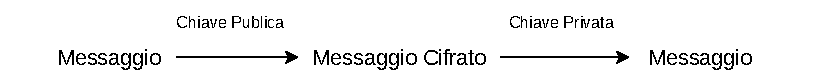
\includegraphics[width=0.9\linewidth]{logos/crit1.pdf}
\end{figure}

Facendo un esempio pratico: supponiamo che abbiamo una rete con 3 computer (chiamiamoli come A, B, C), ciascun dispositivo ha chiaramente una propria chiave publica e una privata, denominiamo $K_a$, $K_b$, $K_c$ le chiavi publiche e $S_a$, $S_b$, $S_c$ le chiavi private ($S$ sta per \textit{secret})




\begin{figure} [h]
    \centering
    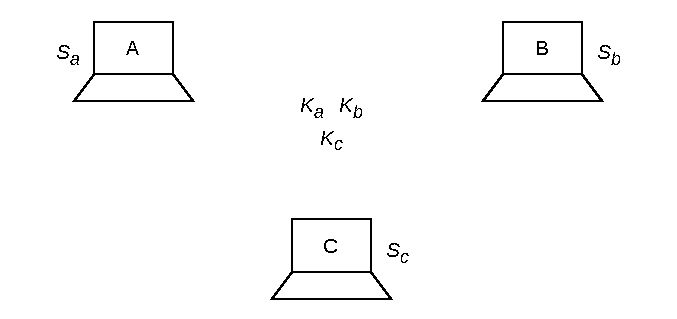
\includegraphics[width=0.7\linewidth]{logos/crit2.pdf}
\end{figure}

Ogni dispositivo conosce la chiave publica (\textbf{K}), mentre tiene per sè la propria chiave publica (\textbf{S})


Supponiamo che il \textbf{PC A} vuole inviare al \textbf{PC B} un pacchetto qualsiasi. Allora il PC A prenderà la chiave publica di B (\textbf{$K_b$}), con quella chiave cripta il messaggio che vuole mandare e lo invierà al PC B.


\begin{figure} [h]
    \centering
    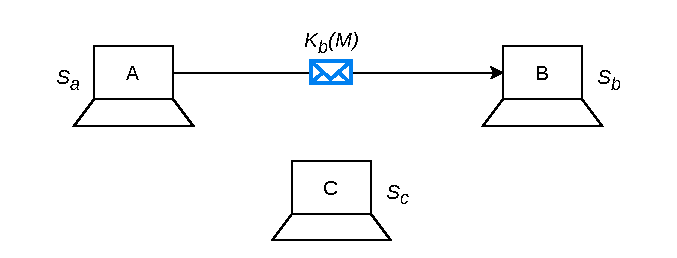
\includegraphics[width=0.7\linewidth]{logos/crit3.pdf}
\end{figure}

Con $M$ si intende il messaggio da inviare e con $K_b(M)$ è il messaggio criptato con la chiave $K_b$. 

In questa maniera se C provasse a intercettare il messaggio non potrà leggere il contenuto perchè è criptato con la chiave publica di B. Solamente B protrà decriptarlo con la sua chiave privata. Se B dovrà rispondere ad A, allora cripterà il messaggio con la chiave publica di A, in modo che solo A protrà decriptarlo. 


\begin{figure} [h]
    \centering
    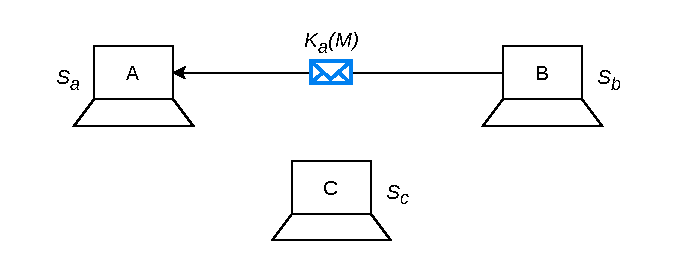
\includegraphics[width=0.7\linewidth]{logos/crit4.pdf}
\end{figure}


Un problema che può nascere da questo algoritmo è se le chiavi publiche sono falsificate. Infatti può succedere che il PC C invia a tutti i una chiave publica dicendo che è quella del PC A, quando invece è la sua. Facendo così i PC che vogliono comunicare con il PC A cripteranno i messaggi con la chiave publica di C (perchè è stata falsificata), e che quindi PC C potrà leggere il messaggio. Per evitare questo problema si usa un altro protocollo, \textbf{Diffie-Hellman} per iniviare le chiavi publiche avendo la certezza che siano del PC corretto.

\newpage
\subsection{Basi di Matematica Modulare}
L'algoritmo RSA è fortemente basato su dei fondamentali di aritmetica modulare molto complessa, quindi prima di descrivere l'algoritmo è meglio ricordare dei principi fondandi di tale algoritmo.

\subsubsection{Aritmetica Modulare}
In primis rivediamo cosa è l'aritmetica modulare. L'aritmetica modulare è quella branca della matematica che studia le operazioni in \textbf{modulo}. Per fare un esempio dobbiamo rivedere come facevamo le divisioni alle elementari, ovvero con il resto. Facciamo la divisione tra 7 e 2.

\begin{equation*}
    \frac{7}{2} = 3 \,\,\, resto \,\,\,  1
\end{equation*}

In aritmetica modulare questa divisione la possiamo scrivere anche nel seguente modo

\begin{equation*}
    7 \equiv 1 \mod 2
\end{equation*}

Si legge "7 è congruo a 1 in modulo 2". Questo vuol dire che se dividiamo 7 per 2 e anche 1 per 2 avranno lo stesso resto (cioè 1). Infatti possiamo dire anche che

\begin{equation*}
    7 \equiv 3 \mod 2
\end{equation*}


Perche anche 3 diviso 2 da come resto 1. Capiamo che con le operaioni modulari a noi interessa soltanto il resto della divisione tra i 2 numeri. Infatti se vogliamo generalizzare, dalla congruenza seguente

\begin{equation*}
    a \equiv b \mod n
\end{equation*}

possiamo affermare che 

\begin{equation}\label{eq:1}
    a = k * n + b
\end{equation}

dove $k$ è un qualsiasi numero, per esempio con la congruenza $ 7 \equiv 3 \mod 2$ possiamo riscriverla come $7 = 2*k + 3$, ed in questo caso $k=2$. Questa proprietà sarà fondamentale per il funzionamento dell'algoritmo

\newpage
\subsubsection{Teoremi Fondamentali}
Per proseguire dobbiamo definire cosa vuole dire che 2 numeri sono \textbf{coprimi}. Due numeri si dicono coprimi se non hanno nessun divisore in comune (apparte 1). In altre parole che il loro massimo comun divisore è 1. Con questa definizione possiamo costruire un insieme molto particolare: $Z_n^*$ (si legge "Zeta n star") dove $n$ è un numero intero positivo. Dato un numero n,   $Z_n^*$ contiene tutti i numeri minori di n coprimi ad n. Per fare chiarezza prendiamo un numero, ad esempio $n=15$. Prendiamo tutti i numeri minori di 15 e scegliamo soltanto quelli che non hanno divisori in comune con 15.


\begin{equation*}
    Z_{15}^* = \{1, 2, 4, 7, 8, 11, 13, 14\}
\end{equation*}

Da notare che se n è un numero primo, allora l'insieme $Z_n^*$ sono tutti i numeri interi positivi minori di n. Ad esempio se $n=7$ allora 

\begin{equation*}
    Z_{7}^* = \{1, 2, 3, 4, 5, 6\}
\end{equation*}


In realtà più che l'insieme in sè a noi interessa quanti numeri ci sono al suo interno. Per farlo c'è una funziona particolare, chiamata \textbf{Funzione Toziente di Eulero}, che dato un numero riesce a calcolare quanti numeri sono coprimi a quel numero. Detto in altre parole, la funzione conta quanti elementi ci sono nell'insieme $Z_n^*$. La funzione viene anche detta \textbf{Funzione $\phi$ di Eulero} perchè viene indicata così $\phi(n)$.


Con l'esempio che abbiamo visto prima, sappiamo che $\phi(15) = 8$, perche se andiamo a contare quanti elementi contiene $Z_{15}^*$ fa proprio 8. Per ora quindi per calcolare La funzione $\phi$ di un numero, prima dobbiamo trovare tutti i numeri coprimi al numero (quindi trovare $Z_n^*$) e calcolare quanti sono i numeri. Però c'è un modo molto più veloce per calcolarlo. Per calcolarlo infatti possiamo scomporre il numero a fattori primi (indicati con la lettera $p$)

\begin{equation*}
    n = p_1 * p_2 * ... *p_k
\end{equation*}
 
 allora

 \begin{equation*}
    \phi(n) = (p_1 - 1) * (p_2 -1)  * ... * (p_k -1 )
\end{equation*}

Tornando al solito esempio di $n=15$


 \begin{equation*}
    15 = 3 * 5
\end{equation*}

allora


 \begin{equation*}
    \phi(15) = (3 - 1) * (5 -1)  = 2 *4 = 8
\end{equation*}

Vediamo che anche con questo metodo $\phi(15) = 8$, semplicemente non abbiamo dovuto calcolare tutti i numeri coprimi ad 15, risparmiandoci così molto tempo.

\newpage
Dalla funzione toziente di Eulero nasce un altro importantissimo teorema: \textbf{Teorema di Eulero aritmetica modulare}, che afferma che dati 2 numeri $a$ e $n$ coprimi tra loro, allora possiamo affermare che:

 \begin{equation}\label{eq:2}
    a^{\phi(n)} \equiv 1 \mod n
\end{equation}

Per capirlo meglio prendiamo il solito esempio con $n=15$. Vuol dire che se prendiamo un qualsiasi numeri coprimo ad 15 (cioè un numero all'interno di $Z_{15}^*$) abbiamo che la divisione per 15 darà resto sempre 1.

Vediamo con 3 numeri coprimi ad 15: $a=2$, $a=7$, $a=13$.

\begin{equation*}
    \frac{a^{\phi(n)}}{n} = \frac{2^8}{15} =  \frac{256}{15} = 17  \,\,\, resto \,\,\, 1
\end{equation*}

\begin{equation*}
    \frac{7^8}{15} =  \frac{5.764.801}{15} = 384.320 \,\,\, resto \,\,\, 1
\end{equation*}

\begin{equation*}
    \frac{13^8}{15} =  \frac{815.730.721}{15} = 54.382.048 \,\,\, resto \,\,\, 1
\end{equation*}

Mentre questa formula non funziona se a e n non sono coprimi. Per vederlo teniamo $n=15$ ma usiamo $a=5$, $a=9$


\begin{equation*}
    \frac{5^8}{15} =  \frac{390.625}{15} = 26.041 \,\,\, resto \,\,\, 10
\end{equation*}

\begin{equation*}
    \frac{9^8}{15} =  \frac{43.046.721}{15} = 2.869.781 \,\,\, resto \,\,\, 6
\end{equation*}


\newpage
\subsection{L'algoritmo}
Dopo aver rivisto tutte le basi neseccarie possiamo vedere come funziona l'algoritmo RSA. Partiamo prendendo 2 numeri primi molto grandi, che chiameremo \textbf{p} e \textbf{q}. Solitamente questi numeri sono a 2048bit, più è grande il numero più è sicuro l'algoritmo. In sucessione definiamo $n$ come

\begin{equation*}
    n = p * q
\end{equation*}

In successione calcoliamo $\phi(n)$, e visto che $n$ è composto da solamente 2 numeri primi (\textbf{p} e \textbf{q} per l'appunto), allora 

\begin{equation*}
    \phi(n) = (p -1 ) * (q -1 )
\end{equation*}


In sucessione scegliamo un numero $e$ che deve essere minore di $\phi(n)$ e coprimo a $\phi(n)$. Spesso viene scelto un numero primo piccolo come $65537$ o qualsiasi altro numero primo piccolo, in modo che siamo sicuri che sia coprimo ad $\phi(n)$. In sucessione calcoliamo il numero $d$ che l'\textbf{inverso modulare} di $e$ in modulo $\phi(n)$, ovvero quel numero che 


\begin{equation*}
    e * d \equiv 1 \mod \phi(n)
\end{equation*}


Per calcolaro si usa l'\textbf{algoritmo di Eulero esteso}, che però in questa dispensa non verrà trattato. A questo punto abbiamo generato le chiavi del nostro algoritmo. La chiave pubblica infatti è data dalla combinazione di (\textbf{n, e}), mentre la chiave privata è la combinazione (\textbf{n, d}). Per trovare il messaggio cifrato (indicato con C) da un messaggio M (che è la rappresentazione numerica di un messaggio, per esempio interpretando i bit del messaggio testuale come se fossero un numero)

\begin{equation*}
    C = M^e \mod n
\end{equation*}


\begin{equation*}
    M = C^d \mod n
\end{equation*}




Un pseudo-codice di un dispositivo che vuole iniziare una comunicazione RSA: 

\begin{lstlisting}[language=CustomPython]
p = numeroPrimo()
q = numeroPrimo()
n = p * q
phi = (p-1) * (q-1)
e = 65557
d = inversoModulare(e, phi)

chiavePublica = (n, e)
chiavePrivata = (n, d)
\end{lstlisting}

\newpage
Supponiamo di inviare una stringa ad un PC qualsiasi (a cui richiederemo la sua chiave publica),Un possibile pseudo-codice per mandare il messaggio:  

\begin{lstlisting}[language=CustomPython]
chiavePublica = richiediChiave()  
messaggio = ""
messCriptato = cripta(messaggio, chiavePublica)
inviaMessaggio(messCriptato)
\end{lstlisting}

Un prossibile script python:

\begin{lstlisting}[language=CustomPython]
n, e = richiediChiave()
messaggio = "Ciao io sono il primo PC"
mess_byte = bytes_to_long(messaggio.encode())
messCriptato = pow(mess_byte, n, e)
print(messCriptato)
\end{lstlisting}

Mentre il pc che riceverà il messaggio per decriptarlo:
\begin{lstlisting}[language=CustomPython]
messCriptato = riceviMessaggio()  
messaggio = decripta(messCriptato, chiavePrivata)
stampa(messaggio)
\end{lstlisting}

in python:
\begin{lstlisting}[language=CustomPython]
messCriptato = riceviMessaggio()
mess = pow(messCriptato, n, d)    
messaggio = long_to_bytes(mess)
print(messaggio)
\end{lstlisting}

\newpage
\subsection{Come mai funziona?}
Per capire come mai funziona questo algoritmo, dobbiamo riprendere l'equazione

\begin{equation*}
    e * d \equiv 1 \mod \phi(n)
\end{equation*}

E grazie all'equazione n\ref{eq:1} sappiamo che possiamo riscriverla nel seguente modo


\begin{equation*}
    e * d = k*\phi(n) + 1 
\end{equation*}


Con k un numero intero positivo, ma non ci interessa il valore. Da questo punto per vedere perchè funziona riprendiamo l'equazione ricordandoci che $C = M^e$


\begin{equation*}
    C^d = (M^e)^d = M^{e*d} \mod n
\end{equation*}

ora possiamo sistituire l'equazione di prima

\begin{equation*}
    M^{e*d} = M^{k*\phi(n) + 1}  = M^{k*\phi(n)} * M^1   =  (M^{\phi(n)})^k * M  \mod n
\end{equation*}

adesso se vediamo la prima parte pella moltiplicazione vediamo che abbiamo $M^{\phi(n)} \mod n$, che  grazie all teorima di Eulero sappiamo, che tutto questo è uguale a 1 in modulo n

\begin{equation*}
   M^{\phi(n)} \equiv 1 \mod n
\end{equation*}

e quindi tornando all'equazione di prima 

\begin{equation*}
   1^k * M \mod n
\end{equation*}

che semplificando viene fuori che 

\begin{equation*}
   C^d =  M \mod n
\end{equation*}



\textbf{N.B.} nel teorema di Eulero chiedeva una restrizione importante, ovvero che M e n siano coprimi tra loro, cosa che ho tralasciato. Questo però non è un problema visto che n è il prodotto di p e q, due numeri primi molto grandi (si parla di numeri anche con 400 cifre), quindi n ha come divisori in comune solo p e q. Pertanto basta che M sia diverso da p e q, ma visto che p e q sono numeri enormi è impossibile che un messaggio sia così tanto grande. Anche lo fosse basta spezzarlo in 2 (o più) messaggi più piccoli.



\newpage
\subsection{Esempio pratico}
Per ricapitolare proviamo a vedere un esempio con dei numeri piccoli a 2 cifre, ma ricordiamoci che nella vita reale i numeri sono molto più grandi.

Prendiamo come numeri $p=61$ e $q=53$ entrambi numeri primi. Con questo possiamo calcolare n e $\phi(n)$

\begin{equation*}
   n = p * q = 61 * 53 = 3233
\end{equation*}

\begin{equation*}
   \phi(3233) = (p -1 ) * (q -1 ) = (61 - 1) * (53 -1) = 3120
\end{equation*}

ora scegliamo un numero e minore di 3120 ($\phi(n)$), per comodità scelgo un numero primo piccolo come $e=17$. Da questo grazie all'algoritmo di Euclide posso calcolare $d=2753$, perchè

\begin{equation*}
   17 * 2753 \equiv 1\mod 3120
\end{equation*}

Ora che abbiamo calcolato tutte le chiavi proviamo a cifrare la lettera \textbf{h}, che secondo la tabella ascii ha valore $M=68$


\begin{equation*}
   C = M^e = 68^{17} \mod 3233 = 1759
\end{equation*}

Ora la nostra lettera cifrata vale $1759$, per decifrare la lettera dobbiamo fare i seguenti calcoli



\begin{equation*}
   M = C^d = 1759^{2753} \mod 3233 = 68
\end{equation*}

Infatti vediamo che siamo tornati al punto di partenza. Per chi avesse molto tempo libero e volesse esercitarsi in questo argomento provare a decifrare il seguente messaggio:

\vspace{0.7cm}

924641044506842334208913942928831562265038398988867352377330263757334761727

\vspace{0.7cm}
I parametri dell'algoritmo sono:

p = 218665744766088631948022385379872054023

q = 183600866011619720100332834729135699401

e = 65537


\newpage
\subsection{Crackabilità}
Con il termine \textit{\textbf{Crackabilità}} intendo la possibilità e la facilità di indovinare la chiave privata di un sistema RSA. Mettiamoci nei panni di un ipotetico hacker che vuole leggere e decriptare i messaggi in una comunicazione RSA. L'hacker in questione avrà a sua disposizione le chiavi publiche dei 2 host, che sono composte da \textbf{n} e \textbf{e}. Ricordiamo che la chiave privata è composta da \textbf{n} e \textbf{d}, e che quindi all'hacker manca soltanto \textbf{d}.

Infatti un attacco possibile è quello di scoprire quanto vale \textbf{d}, per farlo basta vendere come si calcolava. \textbf{d} veniva fuori dalla equazione :

\begin{equation*}
    d * e \equiv 1 \mod \phi(n)
\end{equation*}


 noi però conosciamo \textbf{e} perchè è parte della chiave publica, quindi per trovare \textbf{d} basta sapere quanto vale \textbf{$\phi(n)$}. Ricordiamo l'equazione da dove viene fuori \textbf{$\phi(n)$}:

 \begin{equation*}
     \phi(n) = (p-1) * (q-1)
 \end{equation*}

 dove \textbf{p} e \textbf{q} sono gli unici divisori di \textbf{n}. In più \textbf{n} noi lo conosciamo perchè fa parte della chiave publica. Quindi per trovate quanto vale \textbf{d} basta trovare i divisori di \textbf{n} per poi trovare \textbf{$\phi(n)$} e infine grazie all'algoritmo di Euclide troavre per l'appunto \textbf{d}.

 Chiaramente se fosse così semplice non si userebbe RSA, infatti abbiamo dato per scontato che sia semplice trovare i divisori di un numero. Ricordiamo che noi con RSA stiamo parlando di numeri molto grandi, ma quando dico molto intento MOLTOOOO. Infatti di solito una buona crittografia RSA è composta da numberi di \textbf{2048} bit, che in decimale hanno più o meno 600 cifre. Per scompore numeri così grandi ci vogliono molti secondi, anzi anni.


 Per farvelo capire vi ho portato un mio persolane "studio". Tramite python ho provato a scomporre dei numeri composti da n-bit. Tramite una libreria python (\textbf{Crypto.Util}) ho generato dei numeri casuali partendo da numeri a 3bit, fino a numeri composti da 69bit. 
\begin{center}
    \begin{tikzpicture}
        \begin{axis}[
            xlabel={n-bit},
            ylabel={sec},
            axis lines=middle, % Places axes in the middle with arrows
            enlargelimits, % Adjusts axis limits to fit arrows
            xlabel style={below right}, % Adjust x-axis label position
            ylabel style={above left}, % Adjust y-axis label position
            axis line style={->}, % Adds arrows to the axes
        ]
            \addplot[
                color=maincolor,
                line width=1.5pt             
            ]
            table {dati3.txt};
        \end{axis}
    \end{tikzpicture}
\end{center}


Possiamo notare come il tempo impiegato cresce in maniera esponenziale al crescere dei bit, che era abbastanza plausibile visto che ogni volta che aggiungiamo un bit moltiplichiamo e che quindi a lungo andate diventa esponensiale. La complessita computazionale di individuare se un numero è primo o meno è di \textbf{$O(\sqrt{n})$}.
\newpage
Codice usato per ricavare i dati dal grafico
\begin{lstlisting}[language=CustomPython]
from Crypto.Util import number
import math
import time as t

def isPrime(num):  
    up = math.ceil(math.sqrt(num))
    
    if(num%2 == 0):
        return False

    for i in range(3, up, 2):
        if num%i == 0:
            return False
    return True

f = open("dati.txt", "a")
bits = [x for x in range(2, 70)]
for bit in bits:
    num = number.getPrime(bit)
    start = t.time()
    isPrime(num)
    finish = t.time()
    f.write(f"{bit}\t{finish-start}\n")
\end{lstlisting}

\newpage
\subsection{Un Futuro Problema}
Abbiamo costatato che la sicurezza dell'RSA è dovuta alla difficoltà nel scomporre numeri molto grandi. Però potenzialmente basta avere un pc particolarmente potente e si può rompere l'algoritmo. 

Negli ultimi anni si stanno sviluppando \textbf{I Computer Quantistici}, che non andremo ad analizzare in questo cotso, ma hanno una potentissima caratteristica. Per via della natura di questi computer, possono performare molte operazioni contemporaneamente, dato che un \textbf{qubit} (il bit quantistico) può essere contemporaneamente sia 0 che 1, al contrario di un bit che può essere o solo 1 o solo 0. Due qubit invece rappresentato allo stesso tempo tutte le loro possibili combinazioni (00, 01, 10, 11). 

\begin{equation*}
    |\psi\rangle = c_0|00\rangle + c_1|01\rangle + c_2|10\rangle+ c_3|11\rangle
\end{equation*}



Con questa particolarità noi possiamo eseguire la stessa operazioni su più numeri contemporaneamente. Grazie a questa potentissima caratteristica, \textbf{Peter Shor} nel 1994 invento \textbf{L'algoritmo di Shor}, che permette di fattorizzare un numero con un tempo computazionale \textbf{polinomiale} $O(n^3\log(n))$. Il funzionamento dell'algoritmo è molto complesso ma sfrutta sempre i teoremi che abbiamo visto, specialmente quello di Fermat 

 \begin{equation*}
    g^{r} \equiv 1 \mod N
\end{equation*}

E l'algoritmo si basa fondalmentalmente su indovinare l'esponente (\textbf{r}) e avicinandosi sempre di più al numero effettivo. 

Ad ogni modo questo algoritmo è molto efficiente, ma per fortuna non è ancora utilizzabile perchè non esiste ancora un computer quantistico potente abbastanza. Infatti il numero più grande che un computer quantistico è riuscito a fattorizzare grazie all'algoritmo di Shor è \textbf{21}. Nonostante non sia ancora un problema questo algoritmo, per evitare problemi in futuro si stanno sviluppando algoritmi che siano difficili da decriptare anche per dei computer quantistici. 

\subsubsection{Funzione Zeta Riemann}
Un'altro possibile rischio per la sicurezza dell'Algoritmo RSA è la possibilità che si possa trovare una funzione matematica che riesca a generare tutti i numeri primi. In caso esistesse, renderebbe molto più veloce crackare una chiave RSA, passando da un tempo computazionale esponenziale a lineare $O(n)$, anche più veloce di un computer quantistico. Per fortuna non si è ancora trovato una funziona che permetta tale funzionamento, ma una parte della comunità scientifica sta studiando perchè si suppone che la \textbf{Funzione Zeta di Riemann} (\textbf{$\zeta(s)$}) possa prevedere i numeri primi.

\begin{equation*}
    \zeta(s) = \sum_{n=1}^{\infty}\frac{1}{n^s}
\end{equation*}

Per ora non c'è alcuna dimostrazione a riguardo ma le ricerche sono ancora in atto.
\newpage
\subsection{Principali attacchi RSA}
\textbf{RSA} è un algoritmo sicuro e non cracckabile per i computer d'oggi. Però se non viene usato come si deve permette tramite certe tecniche di rompere la crittografia. Ora vediamo tre principali attacchi che si possono effettuare su una crittografia RSA non usata in maniera appropriata.


\subsubsection{Low public Exponent}
Inizialmente abbiamo detto che l'esponente publico (\textbf{e}) deve essere primo, affinche esista un inverso modulare (\textbf{d}), quindi può anche essere un numero piccolo come \textbf{3}, \textbf{7}, \textbf{11}. Purtroppo però se usiamo un \textbf{e} molto piccolo possiamo inbattere in un problema. Infatti riprendiamo le formule fondamentali di RSA:

\begin{equation*}
    C \equiv  M ^ e \mod n 
\end{equation*}

Se $M^e < n$ allora non verrà mai fatta la riduzione modulare, perchè il numero non supera il modulo. Con questo il messaccio cifrato sarà soltanto $M^e$ e quindi basta invertire la formula per trovare il messaggio in chiaro

\begin{equation*}
    C =  M ^ e 
\end{equation*}

\begin{equation*}
   M = \sqrt[e]{C}
\end{equation*}

Verosimilmente anche scegliendo messaggi molto corti (come i singoli caratteri) può essere rischioso. A questo proposito ho fatto un piccolo studio in merito. Ho analizzato quanti caratteri minimi servono per un messaggio per non riscontrare in questo problema, in base alla grandezza di chiavi (ho scelto 4 valori: chiavi a \textbf{128bit}, \textbf{256bit}, \textbf{512bit},\textbf{1024bit} e \textbf{2048bit}) e in base a un esponente molto piccolo. In altre parole, ho trovato quanti caratteri servono per un messaggio per avere una riduzione e quindi per essere sicuro, perchè altrimenti basta fare la radice e-esima per tornare al messaggio in chiaro originale.


\begin{figure}[h]
    \centering
    \includegraphics[width=0.80\linewidth]{low_exp_graph.pdf}
\end{figure}

Notiamo che per valori molto bassi servono molti caratteri affinchè avvenga la riduzione modulare, e soppratutto più è grande la chiave più caratteri servono. Chiaramente per dei valori normali di \textbf{e}, come 65337, la riduzione avviene anche con un singolo carattere quindi non è un problema, ma se venisse scelto un esponente piccolo abbiamo visto cosa questo comporta.

\subsubsection{P e Q vicini}
Un altro problema che può accadere è qualora \textbf{p} e \textbf{q} fossero valori molto simili. Per capire perchè può essere un problema analiziamo dal punto di vista matematico. Supponiamo che quindi \textbf{p} e \textbf{q} sono molto simili, e che quindi uno dei due numeri è più grande (supponiamo che q sia il più grande, ma chiaramente è indifferente chi sia il più grande).

\begin{equation*}
    q = p + \Delta x
\end{equation*}

Indichiamo con \textbf{$\Delta x$} la differenza tra i due numeri. Ora proviamo a calcolare il modulo \textbf{n}

\begin{equation*}
    n = p *q= p*(p + \Delta x) = p^2 +p\Delta x
\end{equation*}

Ora analiziamo cosa abbiamo scoperto, perchè ricordiamo che \textbf{p} e \textbf{q} sono numeri enormi (inorno alle 300/400 cifre) mentre $\Delta x$ è un numero relativamente piccolo (vedremo dopo quanto piccolo) ma comunque insignificante rispetto a $p^2$ che ha approssimativamente 600/700 cifre. Quindi il termine con il $\Delta x$ lo possiamo anche trascurare

\begin{equation*}
   p^2 +p\Delta x \approx p^2
\end{equation*}

Da questo troviamo che


\begin{equation*}
    n = p^2 +p\Delta x \approx p^2
\end{equation*}

\begin{equation*}
    n \approx p^2
\end{equation*}

E quindi troviamo una approssimazione molto comoda

\begin{equation*}
    p \approx \sqrt{n}
\end{equation*}

Così abbiamo scoperto che la \textbf{radice di n} è un numero molto vicino a \textbf{p}, perciò si possono cercare tutti i numeri primi vicini a $\sqrt{n}$ per trovare p


\begin{figure}[h]
    \centering
    \includegraphics[width=0.60\linewidth]{math (1).pdf}
\end{figure}

Chiaramente più è grande la differenza ($\Delta x$) più sarà difficile e, nei casi reali praticamente impossibile usare questa tecnica. Questa tecnica ha una complessita computazionale $o(\frac{\Delta x}{4})$, quindi linearmente proporzionale.

Per capire bene anche questo attacco ho provato a vedere quanto tempo ci si impiega a fattorizzare un numero grande (\textbf{n}) con questa tecnica, e ho trovato questo grafico


\begin{figure}[h]
    \centering
    \includegraphics[width=0.90\linewidth]{similar_p_q_plot.pdf}
\end{figure}

Notiamo che già con una differenza di 1.000.000 tra i due fattori primi ci si impiega dai 2 minuti a poco meno di 10 minuti. Una differenza di 1.000.000 è veramente poco rispetto ai numeri da 300 cifre, quindi è facile capire che questo attacco non ha una vera e propria implementazione pratica. 


\subsubsection{Stesso N, diversi esponenti}
Supponiamo che una banca debba creare tutte le chiavi per i suoi cliente, visto che la generazione delle chiavi è un processo molto lungo e dispendioso, supponiamo che decida di usare lo stesso modulo (\textbf{n}) e quindi stessi fattori primi (\textbf{p}, \textbf{q}) ma per ogni cliente usare un esponente diverso (\textbf{e} e quindi di conseguenza \textbf{d}). Inizialmente sembra un'idea molto furba perchè con lo stesso modulo (e quindi evitando tutto il processo di generazione di numeri primi enormi) possiamo dando a ciascun cliente un esponente pubblico diverso (chiaramente deve essere un numero primo). 



\begin{figure}[h]
    \centering
    \includegraphics[width=0.9\linewidth]{sim_n.pdf}
\end{figure}


Vediamo come però come è molto rischioso, perchè ognuno ha la sua coppia di chiavi (\textbf{e}, \textbf{n}) e (\textbf{d}, \textbf{n}) ma nessuno conosce i fattori primi, perchè li possiede solo la banca. Quindi con l'attacco che ora vedremo, possiamo \textbf{fattorizzarte n} partendo da \textbf{e}, \textbf{d}. Questo perchè se qualcuno riuscisse a scomporre i fattori primi potrebbe trovare \textbf{$\phi(n)$} e da li trovare tutti gli esponenti privati di tutti, permettendo così di avere tutte le chiavi del sistema.

Per fattorizzare 




\section{Diffie-Hellman}


\section{Elliptic Curve Cryptografy (ECC)}


\end{document}
